%%%%%%%%%%%%%%%%%%%%%%%%%%%%%%%%%%%%%%%%%%%%%%%%%%%%%%%%%%%%%%%%%%%%%%%%%%%%%%%%
%                                                                              %
% The following preamble was originally written by the CSE 379 course staff at %
% the University at Buffalo as a template for lab documentation.               %
%                                                                              %
%%%%%%%%%%%%%%%%%%%%%%%%%%%%%%%%%%%%%%%%%%%%%%%%%%%%%%%%%%%%%%%%%%%%%%%%%%%%%%%%


\documentclass [10pt]{article}
\NeedsTeXFormat{LaTeX2e}
\ProvidesClass{docs}[2017/05/06 Class for writing documentation and reports]

\oddsidemargin=0.0cm
\textwidth=16.5cm
\textheight=22.8cm
\topmargin=-1.0cm

\RequirePackage[utf8]{inputenc}
\RequirePackage{tabularx}
\RequirePackage{fancyhdr}
\RequirePackage{multirow}
\RequirePackage{mathtools}% Loads amsmath
\RequirePackage[hidelinks]{hyperref}
\RequirePackage{graphicx}
\RequirePackage{float}

\pagestyle{fancy}
\fancyhf{}
\renewcommand{\headrulewidth}{1pt}

\RequirePackage{listings}

% the following is needed for syntax highlighting
\RequirePackage{color}
\RequirePackage{lstlangarm} %arm keywords for syntax highlighting
\definecolor{dkgreen}{rgb}{0,0.6,0}
\definecolor{gray}{rgb}{0.5,0.5,0.5}
\definecolor{mauve}{rgb}{0.58,0,0.82}

\lstset{ %
language=[ARM]{Assembler},      % the language of the code
basicstyle=\normalsize,         % the size of the fonts that are used for the code
numbers=left,                   % where to put the line-numbers
numberstyle=\footnotesize\color{gray},  % the style that is used for the line-numbers
stepnumber=1,                   % the step between two line-numbers. If it's 1, each line
% will be numbered
numbersep=5pt,                  % how far the line-numbers are from the code
backgroundcolor=\color{white},  % choose the background color. You must add \RequirePackage{color}
showspaces=false,               % show spaces adding particular underscores
showstringspaces=false,         % underline spaces within strings
showtabs=false,                 % show tabs within strings adding particular underscores
frame=single,                   % adds a frame around the code
rulecolor=\color{white},        % if not set, the frame-color may be changed on line-breaks within not-black text (e.g. commens (green here))
tabsize=2,                      % sets default tabsize to 2 spaces
captionpos=b,                   % sets the caption-position to bottom
breaklines=true,                % sets automatic line breaking
breakatwhitespace=false,        % sets if automatic breaks should only happen at whitespace
title=\lstname,                 % show the filename of files included with \lstinputlisting;
% also try caption instead of title
keywordstyle=\color{blue},          % keyword style
commentstyle=\color{gray},       % comment style
stringstyle=\color{mauve},         % string literal style
escapeinside={\%*}{*)},            % if you want to add a comment within your code
morekeywords={*,...}               % if you want to add more keywords to the set
}





\lhead{anandbal, asingh42}
\rhead{Lab 7: Wee Dig Dug}
\rfoot{\thepage}
\lfoot{R3}

\author{
  Anand Balakrishnan \\ \texttt{anandbal@buffalo.edu}
  \and
  Amrit Pal Singh \\ \texttt{asingh42@buffalo.edu}
}
\title{Wee Dig Dug: Documentations}


\begin{document}

  \maketitle
  \tableofcontents\newpage

  \section{User Guide}

Welcome to \textbf{Wee Dig Dug}, a simplified text-based version of the popular
arcade game \textbf{Dig Dug} by Namco!.  The following project was written in
ARM Assembly for the LPC2138 Education Board, with the ARM7TDMI architecture.

  \subsection{Setup}

  Before playing the game, please make sure of the following:

  \begin{enumerate} 
    \item You are connected to the correct COM port on PuTTy,
          and at a baud rate of \underline{115200 baud}.
    \item Resize the console window to a minimum of $ 30 \text{rows} \times 30 \text{columns} $.
    \item Just enjoy the game.
  \end{enumerate}

  To start playing, just flash the code onto the LPC2138 board.

  \subsection{Instructions}

  You are the character \textbf{\textit{Dug}} and your job is to :

  \begin{enumerate}
    \item Dig through as much of the sand as you can.
    \item Kill all enemies.  
    \item \textbf{You must kill all the enemies withing 2 minutes or else you die}.  
  \end{enumerate}

  You can move \textbf{\textit{Dug}} using the \texttt{W,A,S,D} keys which correspond to 
  \texttt{UP,DOWN,LEFT,RIGHT} respectively and shoot your bullet using \texttt{SPACEBAR}.
  You can use the 5th Momentary Push Button to \texttt{PAUSE} the game whenever you want.




\section{Developer Guide}

\section{Design}

The game is designed based on the \textbf{Model-View-Controller (MVC)} architecture.
This architecture is a common way of designing applications with a User Interface.
In it, each of the following components is responsible for a particular task, and only that component is allowed to perform that task.

\begin{table}[H]
  \centering
  \begin{tabularx}{\textwidth}{|p{3cm}|p{\textwidth -3cm}|}
    \hline \\
    \multirow{2}{*}{Model}  & This is the part of the framework responsible for maintainin the internal representation of the application.                      \\
                            & The \textbf\{Model\} in this game holds the location where sand is present, state of each sprite and state variables of the game. \\
    \hline \\

    \multirow{2}{*}{View}   & The \textbf\{View\} is responsible for rendering the \textbf\{Model\} onto the GUI. \\
                            & It contains routines that display the board, the sprites and the sand on a console screen.                                        \\
\multirow{2}{*}{Controller} & The \textbf\{Controller\} is responsible for handling user input and triggering changes in the \textbf\{Model\}.                  \\
                            & It contains the entry point for the game and interrupt handlers.                                                                 
\end{tabularx}
\end{table}


\begin{figure}[H]
  \centering
  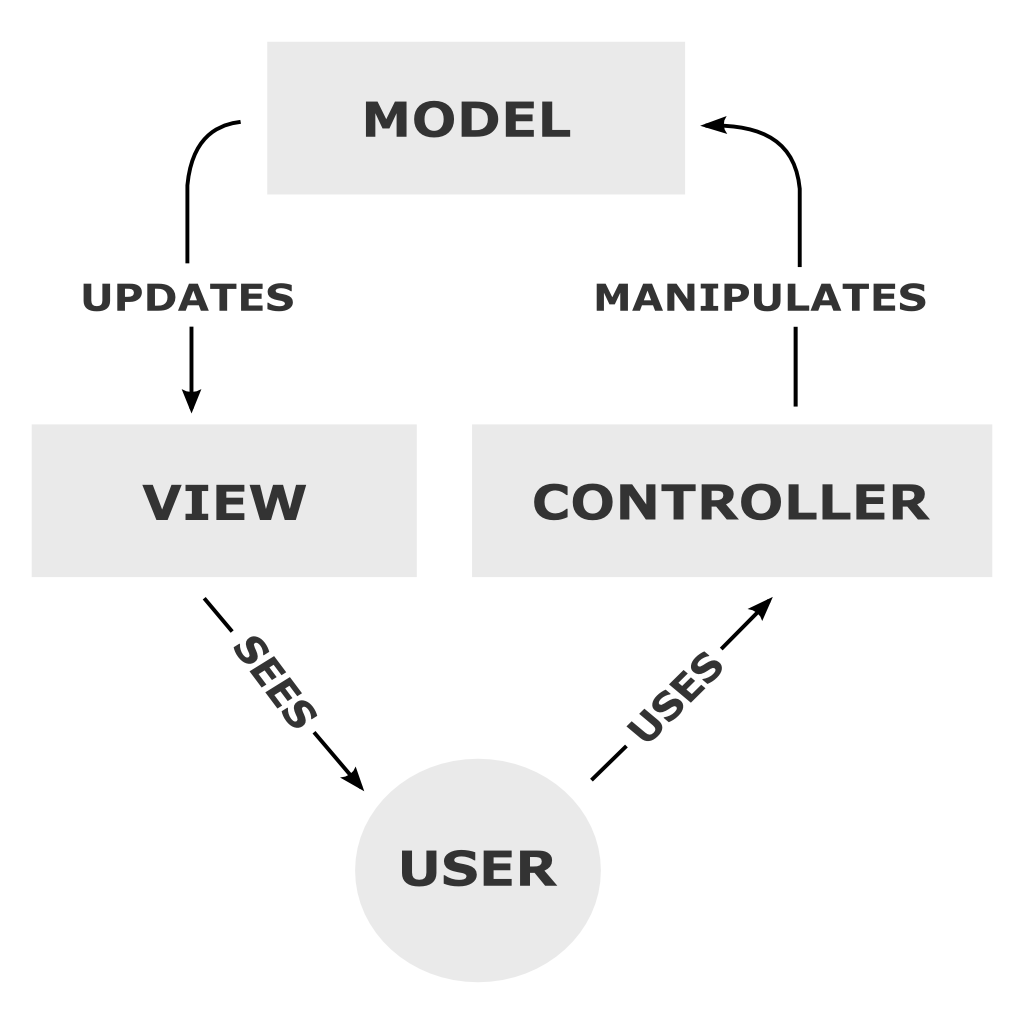
\includegraphics[width=0.5\textwidth]{images/mvc-process.png}
  \caption{\label{fig:mvc-process} The components of the framework interacting with each other (courtsey: Wikipdia)}
\end{figure}

  \subsection{Controller}

  \quad\textbf{FILES}: \texttt{controller.s}

  The \textbf{Controller} mainly contains interrupt handlers, and it is also the entry point for the game.
  In is, we do the following:

  \begin{itemize}
    \item Initialize timer and timer match registers for periodic interrupts.
    \item Listen for UART0 interrupt, read the keystrokes and perform the corresponding action.
    \item Listen for External Interrupt Button press and PAUSE the game.
  \end{itemize}

  The \textbf{Controller} is a relatively small component, responsible mainly for updating the \textbf{Model} via subroutines exposed by the \textbf{Model}.

  \subsection{Model}

  \textbf{FILES}: \texttt{model.s}, \texttt{collisions.s}

  The \textbf{Model} maintains the internal representation of the board and triggers \textbf{View} updates. It exposed routines that allows the
  \textbf{Controller} to trigger updates on the \textbf{Model}.

    \subsubsection{Implementation}

    The \textbf{Model} consists of an \emph{``array''} (created using the \texttt{FILL} directive)
    of size $19 \times 15$ bytes, each byte representing a grain of sand.

    The \textbf{Model} also consists of \texttt{DCD} tables to hold information of sprites. These tables are structured similar to a \texttt{struct}.
    There are also staticaly defined regions of memory that keep track of the various states the game could possibly be in,
    for example, \texttt{PAUSE}, \texttt{GAME\_OVER}.
    The \textbf{Model} is also responsible for keeping track of other variables of the game,
    such as, \texttt{LEVEL}, \texttt{HIGH\_SCORE}, \texttt{CURRENT\_SCORE} and \texttt{TIME}.


    \begin{lstlisting}[float,floatplacement=H,caption={Structure for \texttt{SPRITE} data}]
SPRITE
	DCD X_POS	; Holds X coordinate of the sprite
	DCD Y_POS	; Holds Y coordinate of the sprite
	DCD LIVES	; Holds Number of lives the sprite has
	DCD DIRECTION	; Code for direction the sprite is moving/facing
	DCD OLD_X_POS	; Previous X coordinate of sprite
	DCD OLD_Y_POS	; Previous Y coordinate of sprite
	DCD ORIGINAL_X	; Original X position (to reset when respawning)
	DCD ORIGINAL_Y	; Original Y position (to reset when respawning)

    \end{lstlisting}

    \subsubsection{Operations}

    Operations that are defined by the \textbf{Model} are:

    \begin{itemize}
      \item Initialize and reset model.
      \item Move sprites and update entire model.
      \item Handle and detect collisions.
      \item Get if sand exists at given (x,y) coordinate on the board.
      \item Clear sand at given coordinate (x,y).
      \item Toggle game states (\texttt{BEGIN\_GAME},\texttt{PAUSE}, \texttt{GAME\_OVER}, \texttt{RUNNING}).
      \item Update individual sprites.
      \item Spawn sprites.
    \end{itemize}


  \subsection{View}

  \quad\textbf{FILES}: \texttt{gui.s}, \texttt{peripherals.s}


  The \textbf{View} is responsible for rendering \textbf{Model} onto the GUI. It possessed routines that
  the \textbf{Model} uses to trigger updates to the GUI. This implementation was chosen as updates can
  be triggered as and when the \textbf{Model} is updates.

    \subsubsection{Implementation}


\end{document}
